
\section{Introduction}
Probabilistic sequence modeling plays a crucial role in diverse machine learning applications including natural language processing~\cite{gpt3,peng-etal-2023-rwkv}, video prediction~\cite{ho2022video,yang2023diffusion,flexible_diffusion} and decision making~\cite{openai_dota,dreamer}. 
Next-token prediction models in particular have a number of desirable properties. They enable the generation of sequences with varying length~\cite{10.1162/neco.1997.9.8.1735,818041,DBLP:journals/corr/abs-2006-16236} (generating only a single token or an ``infinite'' number of tokens via auto-regressive sampling), can be conditioned on varying amounts of history~\cite{818041,DBLP:journals/corr/abs-2006-16236}, support efficient tree search\cite{yao2023tree, planet,tdmpc}, and can be used for online feedback control~\cite{dreamer, openai_dota}.

Current next-token prediction models are trained via \emph{teacher forcing}~\cite{teacher_forcing}, where the model predicts the immediate next token based on a ground truth history of previous tokens.
This results in two limitations: (1) there is no mechanism by which one can guide the sampling of a sequence to minimize a certain objective, and
(2) current next-token models easily become \emph{unstable} on continuous data. For example, when attempting to auto-regressively generate a video (as opposed to text~\cite{gpt3} or vector-quantized latents~\cite{hu2023gaia}) past the training horizon, slight errors in frame-to-frame predictions accumulate and the model diverges.

\emph{Full-sequence diffusion} seemingly offers a solution.
Commonly used in video generation and long-horizon planning, one directly models the joint distribution of a fixed number of tokens by diffusing their concatenation~\cite{ho2022video, ajay2022conditional}, where the noise level is identical across all tokens.
They offer \emph{diffusion guidance}~\cite{ho2022classifierfree,dhariwal2021diffusion} to guide sampling to a desirable sequence, invaluable in decision-making (planning) applications~\cite{janner2022planning,huang2023diffusion}. 
They further excel at generating continuous signals such as video~\cite{ho2022video}.
However, full-sequence diffusion is universally parameterized via non-causal, unmasked architectures. 
In addition to restricting sampling to full sequences, as opposed to variable length generation, we show that this limits the possibilities for both guidance and subsequence generation (\Cref{fig:ability}).
Further, we demonstrate that a naive attempt at combining the best of both worlds by training a next-token prediction model for full-sequence diffusion leads to poor generations, intuitively because it does not model the fact that small uncertainty in an early token necessitates high uncertainty in a later one.

In this paper, we introduce \emph{Diffusion Forcing} ({\algshort}), a training and sampling paradigm where each token is associated with a \emph{random, independent} noise level, and where tokens can be denoised according to arbitrary, independent, per-token schedules through a shared next-or-next-few-token prediction model. Our approach is motivated by the observation that noising tokens is a form of \emph{partial masking}---zero noise means a token is unmasked, and complete noise fully masks out a token. Thus, \algshort{} forces the model to learn to ``unmask'' any collection of variably noised tokens (\Cref{fig:method}). Simultaneously, by parameterizing predictions as a composition of next-token prediction models, our system can flexibly generate varying length sequences as well as compositionally generalize to new trajectories (Figure~\ref{fig:ability}).



We implement \algshort{} for sequence generation as \emph{\algoseq{}} ({\algshortseq}), in which future tokens depend on past ones via a causal architecture.
We train the model to denoise all tokens of a sequence at once, with an independent noise level per token. 
During sampling, \algshortseq{} gradually denoises a sequence of Gaussian noise frames into clean samples where different frames may have different noise levels at each denoising step.
Like  next-token prediction models, \algshortseq{} can generate variable-length sequences; unlike next-token prediction, it does so stabily from the immediate next token to thousands of tokens in the future -- even for continuous tokens. Moreover, like full-sequence diffusion it accepts guidance towards high-reward generations. Synergistically leveraging  causality, flexible horizon, and variable noise schedules, \algshortseq{} enables a new capability, 
Monte Carlo Guidance (MCG), that dramatically improves the sampling of high-reward generations   compared to non-causal full-sequence diffusion models.  Fig.~\ref{fig:ability}  overviews these capabilities.
 

\begin{figure}[t]
    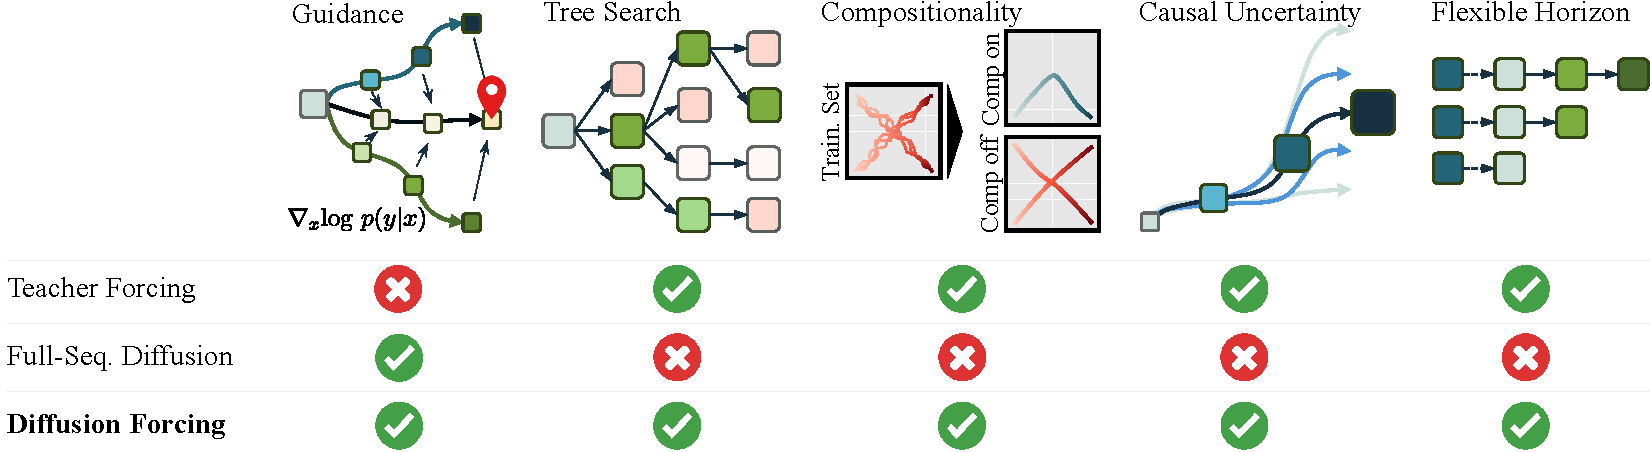
\includegraphics[width=\linewidth]{figures/pdf/Capabilities.pdf}
    \caption{\textbf{\algo{} capabilities.} Today, different applications such as language modeling~\cite{gpt3}, planning~\cite{janner2022planning}, or video generation~\cite{ho2022video,yang2023diffusion} rely on \emph{either} auto-regressive next-token prediction \emph{or} full-sequence diffusion, according to their respective unique capabilities. The proposed \algons{} is a novel sequence generative model that enjoys key strengths of both model types.} 
    \label{fig:ability}
    \vspace{-5pt}
\end{figure}


In summary, our contributions are:
(1) We propose \algons, a new probabilistic sequence model that has the flexibility of next-token prediction models while being able to perform long-horizon guidance like full-sequence diffusion models.
(2) Taking advantage of \algons{}'s unique capabilities, we introduce a novel decision-making framework that allows us to use Diffusion Forcing as simultaneously a \emph{policy} (\cite{chi2023diffusion}) and as a \emph{planner} (\cite{janner2022planning}). 
(3) We formally prove that, under appropriate conditions, optimizing our proposed training objective maximizes a  lower bound on the likelihood of the joint distribution of \emph{all sub-sequences} observed at training time.
(4) We empirically evaluate \algshortseq{} across diverse domains such as video generation, model-based planning, visual imitation learning, and time series prediction, and demonstrate \algshortseq{}'s unique capabilities, such as stabilizing long-rollout autoregressive video generation, composing sub-sequences of those observed at training time with user-determined memory horizon, Monte Carlo Guidance, and more. 


















